Use the college test data in Table 5.2. (See Example 5.5.)
\begin{enumerate}[label= (\alph*)]
    \item Test the null hypothesis $H_{0} : \bm{\mu}^{\prime} = [500, 50, 30]$ versus $H_{1}: \bm{\mu}^{\prime} \ne [500, 50, 30]$ at the
    $\alpha = .05$ level of significance. Suppose ${[ 500, 50, 30]}^{\prime}$ represent average scores for
    thousands of college students over the last 10 years. Is there reason to believe that the
    group of students represented by the scores in Table 5.2 is scoring differently?
    Explain.

    \[
        \bar{\textbf{x}}
        =
        \begin{bNiceArray}{c}
            526.59 \\
             54.69 \\
             25.13
        \end{bNiceArray}
        \hspace{0.2cm}
        \text{and}
        \hspace{0.2cm}
        \textbf{S}
        =
        \begin{bNiceArray}{ccc}
            5808.06 &  597.84 &  222.03 \\
             597.84 &  126.05 &   23.39 \\
             222.03 &  23.39  &   23.11
        \end{bNiceArray}
    \]
    \[
        \textbf{S}^{-1}
        =
        \begin{bNiceArray}{ccc}
             0.00043194 & -0.00157423 & -0.0025565  \\
            -0.00157423 &  0.0155044  & -0.00056675 \\
            -0.0025565  & -0.00056675 &  0.06840139
        \end{bNiceArray}
    \]
    \[
        T^{2}
        =
        n
        {\left(\bar{\textbf{x}} - \bm{\mu}_{0}\right)}^{\prime}
        \textbf{S}^{-1}
        \left(\bar{\textbf{x}} - \bm{\mu}_{0}\right)
        =
    \]
    \begin{multline*}
        =
        87
        {\left(
            \begin{bNiceArray}{c}
                526.59 \\
                 54.69 \\
                 25.13
            \end{bNiceArray}
            -
            \begin{bNiceArray}{c}
                500 \\
                50 \\
                30
            \end{bNiceArray}
        \right)}^{\prime}
        \\
        \times
        \begin{bNiceArray}{ccc}
            0.00043194 & -0.00157423 & -0.0025565  \\
           -0.00157423 &  0.0155044  & -0.00056675 \\
           -0.0025565  & -0.00056675 &  0.06840139
       \end{bNiceArray} \\
       \times
       \left(
            \begin{bNiceArray}{c}
                526.59 \\
                 54.69 \\
                 25.13
            \end{bNiceArray}
            -
            \begin{bNiceArray}{c}
                500 \\
                50 \\
                30
            \end{bNiceArray}
        \right)
        =
    \end{multline*}
    \[
        =
        87
        \begin{bNiceArray}{rrr}
            0.01656039 &  0.03361952 & -0.40398404
        \end{bNiceArray}
        \begin{bNiceArray}{r}
            26.5862069 \\
            4.68965517 \\
            -4.87356322
        \end{bNiceArray}
        =
    \]
    \[
        =
        87(2.56678363)
        =
        223.31
    \]
    Since $T^{2} = 223.31 > \frac{(n-1)p}{n - p} F_{p, n-p} (\alpha) = 8.33$, we would reject the null hypothesis, $H_{0}$, that the mean vector of scores is $[500, 50, 30]$, so one or more of the component means, or combination of means differs from the hypothesized values of $[500, 50, 30]$. If the vector, $[500, 50, 30]$, represents the average score for thousands of college students over the last 10 years, we could say that the scores in table 5.2 are scoring differently. The hypothesized vector lies outside the confidence region for the sample data. There are tons of possibilities for why this happened. There may be sampling bias in Table 5.2 data that isn't present in the larger samle. Also, the size of 87 may contain outliers, or may not be normally distributed. Another possibility may be measurement error in either sample. There also may be some kind of time effect present in either sample as well.

    \item Determine the lengths and directions for the axes of the 95\% confidence ellipsoid for $\bm{\mu}$.
    \newline
    \par
    We have three variables, so our confidence ellipse is a football shape in 3-D.
    The largest eigenvalue is associated with the direction of greatest variability. The largest eigenvalue is $\lambda_{1} = 5878.792$. In the ellipsoid, the half-length of the major axis is $\sqrt{\lambda_{1}}\sqrt{\frac{(n-1)p}{n-p}F_{p, n-p}(\alpha)} = (76.67)(2.89) = 221.34$, so its full length is $2\sqrt{\lambda_{1}}\sqrt{\frac{(n-1)p}{n-p}F_{p, n-p}(\alpha)} = 442.68$, and is in the direction of
    \[
        \textbf{e}_{1}
        =
        \begin{bNiceArray}{c}
            0.99390539 \\
            0.10344339 \\
            0.03809906
        \end{bNiceArray}
    \]
    The second largest eigenvalue is $\lambda_{2} = 63.835$. In the ellipsoid, the half-length of the intermediate axis is $\sqrt{\lambda_{2}}\sqrt{\frac{(n-1)p}{n-p}F_{p, n-p}(\alpha)} = (7.99)(2.89) = 23.06$, so its full length is $2\sqrt{\lambda_{2}}\sqrt{\frac{(n-1)p}{n-p}F_{p, n-p}(\alpha)} = 46.13$, and is in the direction of
    \[
        \textbf{e}_{2}
        =
        \begin{bNiceArray}{r}
             0.10373153 \\
            -0.99458923 \\
            -0.00566024
        \end{bNiceArray}
    \]
    The smallest eigenvalue is associated with the direction of least variability. The smallest eigenvalue is $\lambda_{3} = 14.598$. In the ellipsoid, the half-length of the minor axis is $\sqrt{\lambda_{2}}\sqrt{\frac{(n-1)p}{n-p}F_{p, n-p}(\alpha)} = (3.82)(2.89) = 11.03$, so its full length is $2\sqrt{\lambda_{3}}\sqrt{\frac{(n-1)p}{n-p}F_{p, n-p}(\alpha)} = 22.06$, and is in the direction of
    \[
        \textbf{e}_{3}
        =
        \begin{bNiceArray}{r}
            -0.0373074  \\
            -0.00957782 \\
             0.99925794 
        \end{bNiceArray}
    \]
    
    \item Construct \textit{Q-Q} plots from the marginal distributions of social science and history,
    verbal, and science scores. Also, construct the three possible scatter diagrams from
    the pairs of observations on different variables. Do these data appear to be normally
    distributed? Discuss.

    \begin{figure}[H]
        \centering
        \begin{tabular}{cc}
            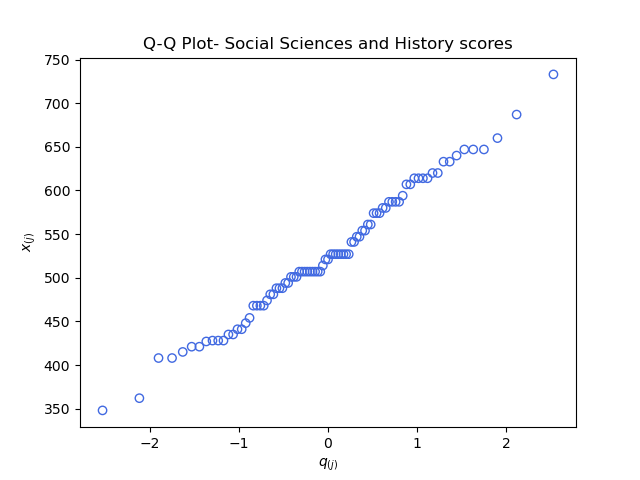
\includegraphics[scale=0.35]{./python/chapter-5/Question-5-18-c-QQ-SocSciHist.png} &
            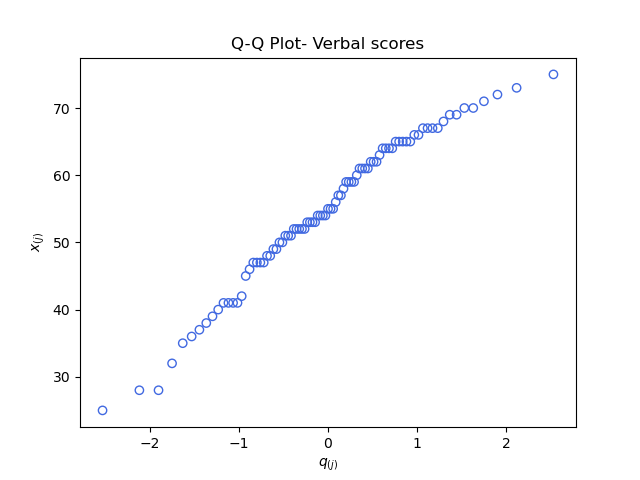
\includegraphics[scale=0.35]{./python/chapter-5/Question-5-18-c-QQ-Verbal.png} \\
            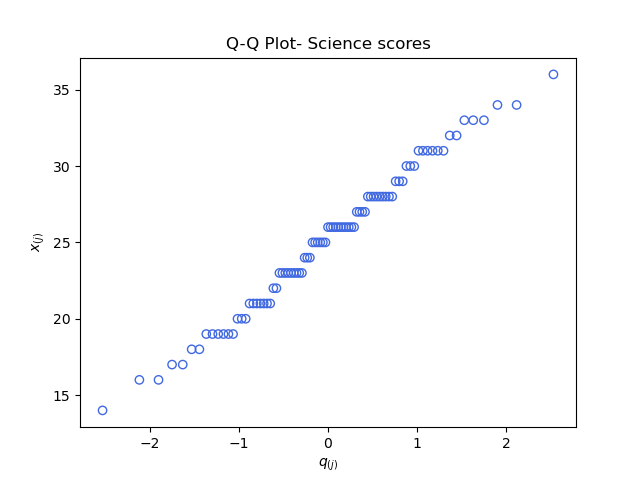
\includegraphics[scale=0.35]{./python/chapter-5/Question-5-18-c-QQ-Science.png}
        \end{tabular}
    \end{figure}

    \begin{figure}[H]
        \centering
        \begin{tabular}{cc}
            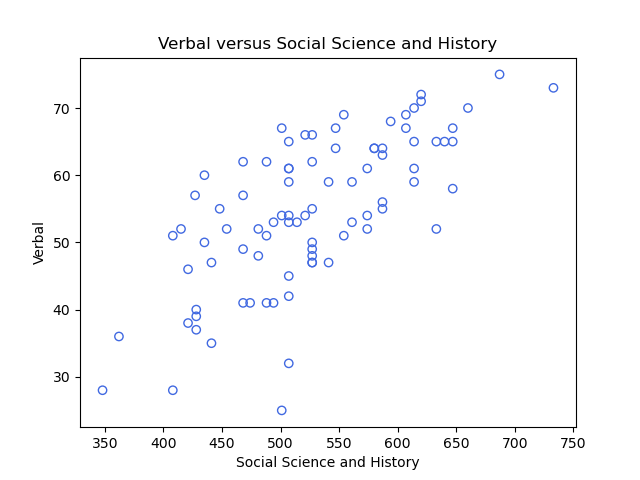
\includegraphics[scale=0.35]{./python/chapter-5/Question-5-18-c-xy-SocSciHist-Verbal.png} &
            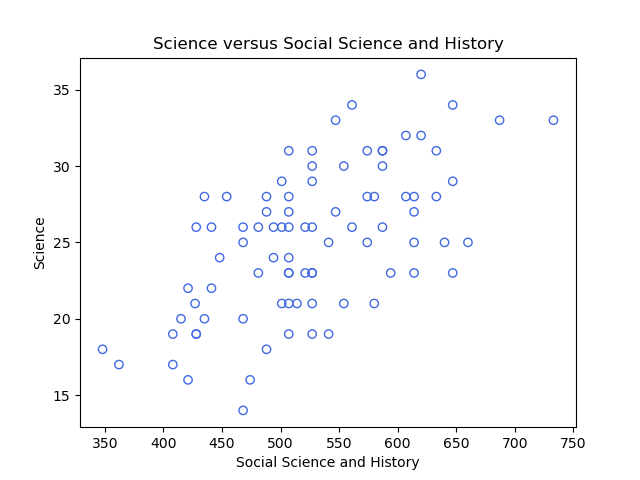
\includegraphics[scale=0.35]{./python/chapter-5/Question-5-18-c-xy-SocSciHist-Science.png} \\
            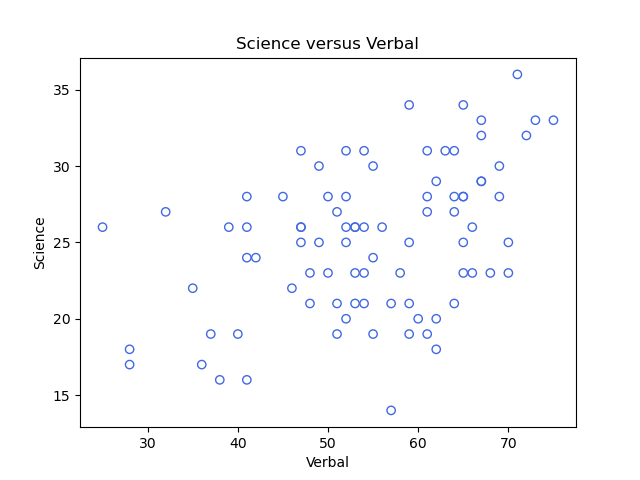
\includegraphics[scale=0.35]{./python/chapter-5/Question-5-18-c-xy-Verbal-Science.png}
        \end{tabular}
    \end{figure}
\end{enumerate}

Just at a glance the \textit{Q-Q} look alright. The plots for social sciences and history and science alone look great. The verbal scores plot does show a slight curve in the right tail, but nothing crazy. The 2-D scatterplots of the data do show positive correlations. The plot of science versus verbal appears to be the weakest. Overall, I'd say these look okay.
